\documentclass[tikz,border=8pt]{standalone}
\usepackage{amsmath}\usepackage{pgfplots}
\pgfplotsset{compat=1.18}
\definecolor{ink}{HTML}{21352F}\definecolor{teal}{HTML}{087F7B}\definecolor{gold}{HTML}{C58B2A}\definecolor{rose}{HTML}{B65A62}\definecolor{blue}{HTML}{4B77A8}
\begin{document}
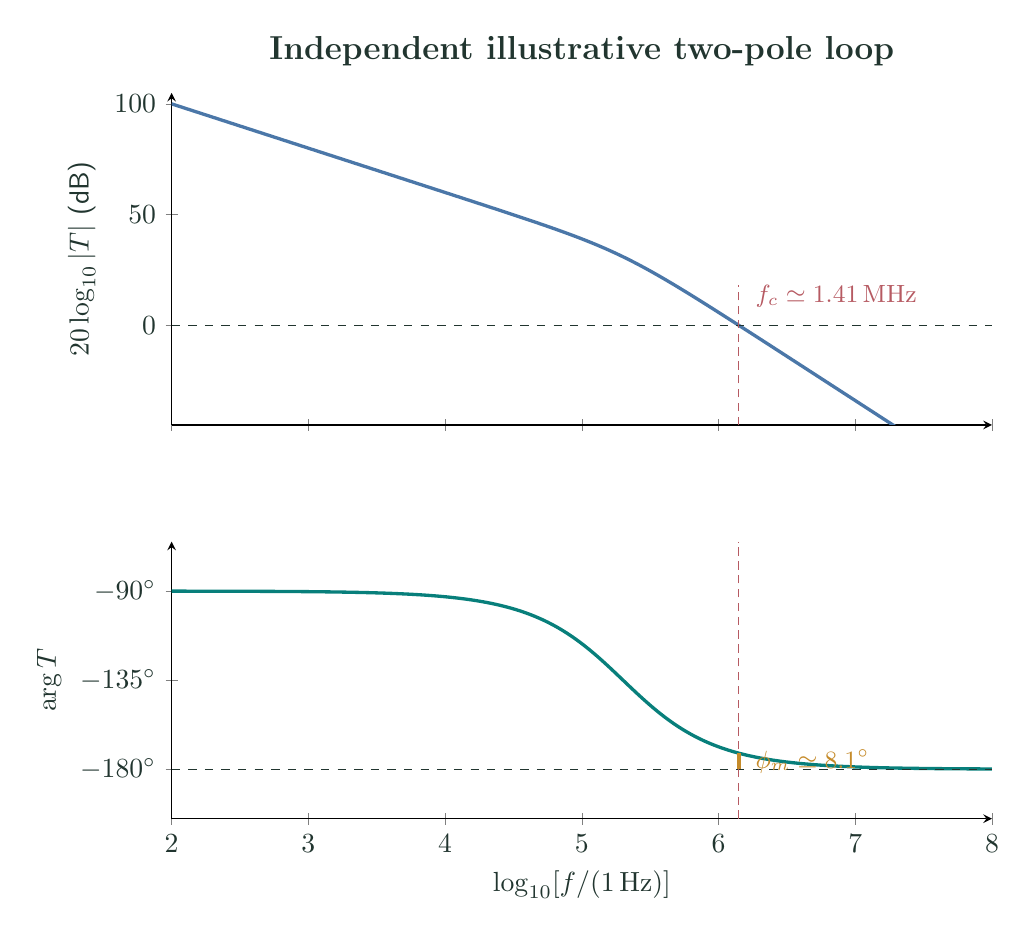
\begin{tikzpicture}[font=\sffamily,text=ink]
\begin{axis}[at={(0,0)},anchor=south west,width=12cm,height=5.8cm,xmin=2,xmax=8,ymin=-45,ymax=105,axis lines=left,ylabel={$20\log_{10}|T|$ (dB)},xticklabels=\empty,title={Independent illustrative two-pole loop},title style={font=\bfseries\large}]
 \addplot[blue,very thick,domain=2:8,samples=300] {100-20*(x-2)-10*log10(1+(10^x/2e5)^2)};
 \addplot[ink,dashed] coordinates {(2,0)(8,0)};
 \addplot[rose,densely dashed] coordinates {(6.149,-45)(6.149,18)};
 \node[rose,font=\small,anchor=west] at (axis cs:6.2,13) {$f_c\simeq1.41\,\mathrm{MHz}$};
\end{axis}
\begin{axis}[at={(0,-5cm)},anchor=south west,width=12cm,height=5.1cm,xmin=2,xmax=8,ymin=-205,ymax=-65,axis lines=left,xlabel={$\log_{10}[f/(1\,\mathrm{Hz})]$},ylabel={$\arg T$},ytick={-180,-135,-90},yticklabels={$-180^\circ$,$-135^\circ$,$-90^\circ$}]
 \addplot[teal,very thick,domain=2:8,samples=300] {-90-atan(10^x/2e5)};
 \addplot[ink,dashed] coordinates {(2,-180)(8,-180)};
 \addplot[rose,densely dashed] coordinates {(6.149,-205)(6.149,-65)};
 \addplot[gold,very thick] coordinates {(6.149,-180)(6.149,-171.9)};
 \node[gold,font=\small,anchor=west] at (axis cs:6.2,-176) {$\phi_m\simeq8.1^\circ$};
\end{axis}
\end{tikzpicture}
\end{document}
